%%%%%%%%%%%%%%%%%%%%%%%%%%%%%%%%%%%%%%%%%%%%%%%%%%
\begin{frame}[fragile]{\de{Funktional, das ist doch nur für Esoteriker?!}\en{Functional, isn't that a totally esoteric subject?!}}

\onslide+<2>
\begin{itemize}
\de{
\item ABN AMRO Amsterdam \textcolor{gray}{\textit{Risikoanalysen Investmentbanking}}
\item AT\&T \textcolor{gray}{\textit{Netzwerksicherheit: Verarbeitung von Internet-Missbrauchsmeldungen}}
\item Bank of America Merril Lynch \\ \textcolor{gray}{\textit{Backend: Laden \& Transformieren von Daten}}
\item Barclays Capital Quantitative Analytics Group \\ \textcolor{gray}{\textit{Mathematische Modellierung von Derivaten}}
\item Bluespec, Inc. \textcolor{gray}{\textit{Modellierung \& Verifikation integrierter Schaltkreise}}
\item Credit Suisse \textcolor{gray}{\textit{Prüfen und Bearbeiten von Spreadsheets}}
\item Deutsche Bank Equity Proprietary Trading, Directional Credit Trading \textcolor{gray}{\textit{Gesamte Software-Infrastruktur}}
\item Facebook \textcolor{gray}{\textit{Interne Tools}}
\item Factis Research, Freiburg \textcolor{gray}{\textit{Mobil-Lösungen (Backend)}}
\item fortytools gmbh \textcolor{gray}{\textit{Webbasierte Produktivitätstools - REST-Backend}}
\item Functor AB, Stockholm \textcolor{gray}{\textit{Statische Codeanalyse}}
}
\en{
\item ABN AMRO Amsterdam \textcolor{gray}{\textit{Risk analysis in investment banking}}
\item AT\&T \textcolor{gray}{\textit{Network security: processing of internet abuse complaints}}
\item Bank of America Merril Lynch \\ \textcolor{gray}{\textit{Backend data transformation and loading}}
\item Barclays Capital Quantitative Analytics Group \\ \textcolor{gray}{\textit{Mathematical modelling of equity derivatives}}
\item Bluespec, Inc. \textcolor{gray}{\textit{Modelling \& verification of integrated circuits}}
\item Credit Suisse \textcolor{gray}{\textit{Checking, manipulating and transforming spreadsheets}}
\item Deutsche Bank Equity Proprietary Trading, Directional Credit Trading \textcolor{gray}{\textit{All its software infrastructure}}
\item Facebook \textcolor{gray}{\textit{Internal tools}}
\item Factis Research, Freiburg \textcolor{gray}{\textit{Mobile solutions (backend)}}
\item fortytools gmbh \textcolor{gray}{\textit{web-based productivity tools - REST-backend}}
\item Functor AB, Stockholm \textcolor{gray}{\textit{static analysis}}
}
\end{itemize}
\end{frame}

\begin{frame}[fragile]{\de{Funktional, das ist doch nur für Esoteriker?!}\en{Functional, isn't that a totally esoteric subject?!}}
\begin{itemize}
\de{
\item Galois, Inc \textcolor{gray}{\textit{Security, Informationssicherheit, Kryptographie}}
\item Google \textcolor{gray}{\textit{Interne Projekte}}
\item IMVU, Inc. \textcolor{gray}{\textit{Social entertainment}}
\item JanRain \textcolor{gray}{\textit{Netzwerk- und Web-Software}}
\item MITRE \textcolor{gray}{\textit{Analyse kryptographischer Protokolle}}
\item New York Times \textcolor{gray}{\textit{Bildverarbeitung für die New York Fashion Week}}
\item NVIDIA \textcolor{gray}{\textit{In-House Tools}}
\item Parallel Scientific \textcolor{gray}{\textit{Hochskalierbares Cluster-Verwaltungssystem}}
\item Sankel Software \textcolor{gray}{\textit{CAD/CAM, Spiele, Computeranimation}}
\item Silk, Amsterdam \textcolor{gray}{\textit{Filtern und Visualisieren großer Datenmengen}}
\item Skedge Me \textcolor{gray}{\textit{Online-Terminvereinbarungen}}
\item Standard Chartered \textcolor{gray}{\textit{Bankensoftware}}
\item Starling Software, Tokio \textcolor{gray}{\textit{Automatisiertes Optionshandelssystem}}
\item Suite Solutions \textcolor{gray}{\textit{Verwaltung technischer Dokumentationen}}
}
\en{
\item Galois, Inc \textcolor{gray}{\textit{Security, information assurance and cryptography}}
\item Google \textcolor{gray}{\textit{Internal projects}}
\item IMVU, Inc. \textcolor{gray}{\textit{Social entertainment}}
\item JanRain \textcolor{gray}{\textit{Network and web software}}
\item MITRE \textcolor{gray}{\textit{Analysis of kryptographic protocols}}
\item New York Times \textcolor{gray}{\textit{Image processing for the New York Fashion Week}}
\item NVIDIA \textcolor{gray}{\textit{In-house tools}}
\item Parallel Scientific \textcolor{gray}{\textit{High-availability cluster management system}}
\item Sankel Software \textcolor{gray}{\textit{CAD/CAM, gaming and computer animation}}
\item Silk, Amsterdam \textcolor{gray}{\textit{Filter and visualize large amounts of information}}
\item Skedge Me \textcolor{gray}{\textit{Online scheduling platform}}
\item Standard Chartered \textcolor{gray}{\textit{Wholesale banking business}}
\item Starling Software, Tokio \textcolor{gray}{\textit{Commercial automated options trading system}}
\item Suite Solutions \textcolor{gray}{\textit{Management of large sets of technical documentation}}
}
\end{itemize}
{\small (Quelle: \url{http://www.haskell.org/haskellwiki/Haskell_in_industry})}
\end{frame}


%%%%%%%%%%%%%%%%%%%%%%%%%%%%%%%%%%%%%%%%%%%%%%%%%%
\begin{frame}[fragile]{\de{Bekannte funktionale Sprachen}\en{Well-known functional languages}}
\begin{tikzpicture}
\draw (1.5, 1.5) node {Lisp};
\draw (1.5, 5.5) node {Scheme};
\draw (4.2, 4.9) node {ML};
\draw (10.5, 3.5) node {OCaml};
\draw (1.5, 3.5) node {Miranda};
\draw (7.3, 4.6) node {F\#};
\draw (6.3, 5.6) node {Erlang};
\draw (9.3, 5.3) node {Clojure};
\draw (4.5, 1.5) node {Scala};

\onslide+<1-2>
\draw (5.5, 3.0) node {Haskell};
\onslide+<2>
\draw (8.5, 1.3) node {(JavaScript)};
\draw (8.1, 2.7) node {(Java 8)};
\onslide+<3>
\draw (5.5, 3.0) node {\color{red}Haskell};
\draw (8.5, 1.3) node {\js{\color{red}}(JavaScript)};
\draw (8.1, 2.7) node {\java{\color{red}}(Java 8)};
\end{tikzpicture}

\end{frame}

%%%%%%%%%%%%%%%%%%%%%%%%%%%%%%%%%%%%%%%%%%%%%%%%%%
\begin{frame}[fragile]{\de{Was ist denn an funktionaler Programmierung so besonders?}\en{Now, what is so special about functional programming?}}

\onslide+<2->
\begin{center}
\LARGE
Immutability
\end{center}

\begin{itemize}
\onslide+<3->
\item \de{Jeder Variablen darf nur einmal ein Wert zugewiesen werden}
\en{Each variable can only be assigned to once}

\onslide+<4->
\item \de{In Java nicht direkt unterstützt} \en{Not directly supported in Java}

\onslide+<5->
\item \de{Kann trotzdem leicht verwirklicht werden:} \en{Can easily be put into effect:}
\end{itemize}

\begin{lstlisting}{Java}
class Point {
  private final int x, y;
  public Point (int x, int y) {
    this.x = x;
    this.y = y;
  }
  // only read x and y in the remaining code
}
\end{lstlisting}


\end{frame}



%%%%%%%%%%%%%%%%%%%%%%%%%%%%%%%%%%%%%%%%%%%%%%%%%%
\begin{frame}[fragile]{\de{Was ist denn an funktionaler Programmierung so besonders?}\en{Now, what is so special about functional programming?}}

\begin{center}
\LARGE
\de{Seiteneffektfreiheit} \en{Absence of side-effects}
\end{center}

\begin{itemize}
\onslide+<2->
\item \de{\glqq{}alles, was den Ablauf eines Computerprogramms oder die Außenwelt verändert, ohne von einer Funktion zurückgegeben worden zu sein\grqq{}} \en{``everything that changes the execution of a computer program or the outside world without being returned from a function''}

\onslide+<3->
\begin{itemize}
\item \de{Ein-/Ausgabe} \en{Input and output}
\item \de{Exceptions} \en{Exceptions}
\item \de{Logging} \en{Logging}
\item \de{Abhängigkeit von (externen) Konfigurationen} \en{Dependency on (external) configurations}
\item \de{Veränderungen des Zustands} \en{Change of state}
\item \de{Nichtdeterminismus (z. B. durch die Verwendung eines Zufallszahlengenerators)} \en{Nondeterminism (e.g.~use of a random number generator)}
\end{itemize}

\onslide+<4->
\item \de{Manche Sprachen zeigen das Vorhandensein von Seiteneffekten sogar in der Typsignatur an} \en{Some languages even indicate side-effects in the type signature}

\end{itemize}


\end{frame}

%%%%%%%%%%%%%%%%%%%%%%%%%%%%%%%%%%%%%%%%%%%%%%%%%%
\begin{frame}[fragile]{\de{Was ist denn an funktionaler Programmierung so besonders?}\en{Now, what is so special about functional programming?}}

\begin{center}
\LARGE
\de{Seiteneffektfreiheit} \en{Absence of side-effects}
\end{center}

\de{auch nicht direkt durch Java 8 unterstützt - Codierungsregeln helfen} 
\en{not directly supported by Java 8 either - coding rules help}

~\\

\onslide+<2->
\begin{lstlisting}{Java}
class SeparationOfSideEffects {

  public void withSideEffect(){
    String initialValue = System.console().readLine(); 
    String result = withoutSideEffect(initialValue);
    System.out.println("The Result: " + result);
  }

  public static String withoutSideEffect(String initialValue){
    return /* function result */ ;
  }
}
\end{lstlisting}

\end{frame}

%%%%%%%%%%%%%%%%%%%%%%%%%%%%%%%%%%%%%%%%%%%%%%%%%%
\begin{frame}[fragile]{\de{Was ist denn an funktionaler Programmierung so besonders?}\en{Now, what is so special about functional programming?}}

\begin{center}
\LARGE
\de{Funktionen sind}\en{Functions are} \glqq{}first order citizens\grqq{}
\end{center}

\onslide+<2->
\begin{center}
\de{Mit Funktionen kann man dasselbe machen wie mit Strings oder Zahlen}
\en{Functions can be treated in the same way as strings or numbers}
\end{center}

\end{frame}

%%%%%%%%%%%%%%%%%%%%%%%%%%%%%%%%%%%%%%%%%%%%%%%%%%
% Unterschiedlich!!
\begin{frame}[fragile]{\de{Funktionen sind Werte}\en{Functions are values}}
\onslide*<2>{
Java 8: \de{Statische Methoden}\en{Static Methods}
% lstinputlisting ist erforderlich wegen onslide* !!
\lstinputlisting[language=Java]{funktionenSindWerte1.txt}
}
\onslide*<3>{
Java 8: \de{Objektmethoden}\en{Object methods}
\lstinputlisting[language=Java]{funktionenSindWerte2.txt}
}
\onslide*<4>{
Java 8: Lambdas
\lstinputlisting[language=Java]{funktionenSindWerte3.txt}
}
\onslide+<5->
Java 8: Lambdas \de{(mit eigenem Funktionsinterface)}\en{(with self-defined function interface)}
\begin{lstlisting}{Java}
interface TimesFunction { int eval(int x, int y); }

TimesFunction times = (x, y) -> x * y;

times.eval(3, 5);                                    // 15
\end{lstlisting}
\onslide+<6->
Haskell:
\begin{lstlisting}{Haskell}
times x y = x * y

timesVar = times

timesVar 3 5                                        -- 15
\end{lstlisting}

\end{frame}

%%%%%%%%%%%%%%%%%%%%%%%%%%%%%%%%%%%%%%%%%%%%%%%%%%
% Unterschiedlich!!
\begin{frame}[fragile]{\de{Funktionen sind Funktionsparameter}\en{Functions are function parameters}}
\onslide+<2->
Java 8:
\begin{lstlisting}{Java}
class Examples { 
    static int apply(IntUnaryOperator func, int arg) { 
        return func.applyAsInt(arg); 
    }
}

Examples.apply(x -> 3 * x, 5);                 // 15
\end{lstlisting}

\onslide+<3->
Haskell:
\begin{lstlisting}{Haskell}
apply func arg = func arg

apply (\ x -> 3 * x) 5                         -- 15
\end{lstlisting}

\end{frame}

%%%%%%%%%%%%%%%%%%%%%%%%%%%%%%%%%%%%%%%%%%%%%%%%%%
% Unterschiedlich!!
\begin{frame}[fragile]{\de{Funktionen sind Rückgabewerte}\en{Functions are return values}}
\onslide+<2->
Java 8:
\begin{lstlisting}{Java}
interface FunctionFunction { IntUnaryOperator eval(int x); }

FunctionFunction times = x -> { return y -> x * y; };

times.eval(3).applyAsInt(5);                    // 15
\end{lstlisting}

\onslide+<3->
Haskell:
\begin{lstlisting}{Haskell}
times x = (\y -> x * y)

times 3 5                                       -- 15
\end{lstlisting}

\end{frame}

%%%%%%%%%%%%%%%%%%%%%%%%%%%%%%%%%%%%%%%%%%%%%%%%%%
% Unterschiedlich!!
\begin{frame}[fragile]{\de{Komisch, oder?}\en{Strange... ?!}}
Java 8: \de{Zwei verschiedene Aufrufe}\en{Two different invocations}
\begin{lstlisting}{Java}
IntBinaryOperator times = (x, y) -> x * y;
times.applyAsInt(3, 5);                                   // 15

FunctionFunction times = x -> { return y -> x * y; };
times.eval(3).applyAsInt(5);                              // 15
\end{lstlisting}
~\\
Haskell: \de{Zweimal derselbe Aufruf}\en{Two identical invocations}
\begin{lstlisting}{Haskell}
times x y = x * y
times 3 5                                                 -- 15

times x = (\y -> x * y)
times 3 5                                                 -- 15
\end{lstlisting}

\end{frame}

%%%%%%%%%%%%%%%%%%%%%%%%%%%%%%%%%%%%%%%%%%%%%%%%%%
\begin{frame}[fragile]{Currying! (\de{oder auch Schönfinkeln}\en{also known as Schönfinkeling})}
\onslide+<2->
\de{In manchen funktionalen Sprachen schreiben wir:}\en{In some functional languages we write:}
\begin{lstlisting}{Haskell}
times x y = x * y
\end{lstlisting}

\de{und eigentlich passiert Folgendes:}\en{but actually the following happens:}
\begin{lstlisting}{Haskell}
times x = (\y -> x * y)
\end{lstlisting}

\onslide+<3->
\de{Denn: Funktionen haben immer genau ein Argument}\en{Because functions always take exactly one argument}
\vfill
\onslide+<4->
\de{Nutzen: Partielle Evaluierung:}\en{Useful for partial evaluation:}
\begin{lstlisting}{Haskell}
times x y = x * y

times3 = times 3

times3 5                          -- 15
\end{lstlisting}


\end{frame}

%%%%%%%%%%%%%%%%%%%%%%%%%%%%%%%%%%%%%%%%%%%%%%%%%%
% Unterschiedlich!!
\begin{frame}[fragile]{\de{Wichtige Bibliotheksfunktionen}\en{Important library functions}: filter}
\begin{itemize}
\item filter \de{oder auch}\en{or} select
\onslide+<2->
\item \de{Nimmt eine Collection und eine Funktion}\en{Takes a collection and a function}
\item \de{Liefert diejenigen Elemente der Collection, für die die Funktion \texttt{true} ergibt}\en{Returns those elements of the collection for which the function yields \texttt{true}}
\end{itemize}

\onslide+<3->
Java 8:
\begin{lstlisting}{Java}
Stream<Integer> filteredStream = 
        asList(1, 2, 3, 4).stream().filter(x -> x % 2 == 0);

filteredStream.toArray();                          // new Integer[]{2, 4}
filteredStream.collect(Collectors.toList());       // Liste mit 2 und 4
\end{lstlisting}

\onslide+<4->
Haskell:
\begin{lstlisting}{Haskell}
filter (\x -> x `mod` 2 == 0) [1,2,3,4]                         -- [2,4]
\end{lstlisting}

\end{frame}

% find oder detect

%%%%%%%%%%%%%%%%%%%%%%%%%%%%%%%%%%%%%%%%%%%%%%%%%%
% Unterschiedlich!!
\begin{frame}[fragile]{\de{Wichtige Bibliotheksfunktionen}\en{Important library functions}: map}
\begin{itemize}
\item map \de{oder auch}\en{or} collect
\onslide+<2->
\item \de{Nimmt eine Collection und eine Funktion}\en{Takes a collection and a function}
\item \de{Liefert eine Collection, in der die Funktion auf jedes Element der ursprünglichen Collection angewandt wurde}\en{Yields a collection of the results of applying the function to the elements of the original collection}
\end{itemize}

\onslide+<3->
Java 8:
\begin{lstlisting}{Java}
Arrays.asList(1, 2, 3, 4).stream().map(x -> x + 5).toArray();                                       // new Integer[]{6, 7, 8, 9}
\end{lstlisting}

\onslide+<4->
Haskell:
\begin{lstlisting}{Haskell}
map (\x -> x + 5) [1,2,3,4]                               -- [6,7,8,9]
\end{lstlisting}

\end{frame}

%%%%%%%%%%%%%%%%%%%%%%%%%%%%%%%%%%%%%%%%%%%%%%%%%%
% Unterschiedlich !!
\begin{frame}[fragile]{\de{Wichtige Bibliotheksfunktionen}\en{Important library functions}: reduce}
\begin{itemize}
\item reduce \de{oder auch}\en{or} foldl / foldr \de{oder}\en{or} inject
\onslide*<2>{
\item \de{Nimmt eine Collection, eine Funktion und einen Startwert}\en{Takes a collection, a function and an initial value}
\item \de{Verbindet Startwert und erstes Element der Collection mit Hilfe der Funktion}\en{Merges initial value and first collection entry using the function}
\item \de{Verbindet das Ergebnis mit dem nächsten Element der Collection}\en{Merges the result and the next collection entry}
\item \de{Setzt dies für alle Elemente der Collection fort, bis nur noch ein Element übrigbleibt}\en{Continues for all collection entries, yielding a single result}
}
\end{itemize}

\onslide+<3->

Java 8:
\begin{lstlisting}{Java}
Arrays.asList(2, 3, 4, 5).stream().reduce(1, (x, y) -> x*y);         // 120
\end{lstlisting}
\onslide+<4->
Haskell:
\begin{lstlisting}{Haskell}
foldl	(*) 1 [2,3,4,5]                                                -- 120
\end{lstlisting}

\onslide+<3->
\begin{center}
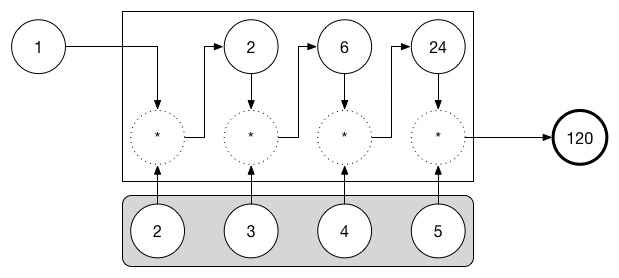
\includegraphics[width=.7\framewidth]{fold_1.png}
\end{center}

\end{frame}

%%%%%%%%%%%%%%%%%%%%%%%%%%%%%%%%%%%%%%%%%%%%%%%%%%
\begin{frame}[fragile]{\de{Typinferenz}\en{Type Inference}}
\begin{itemize}
\item Haskell: \de{starkes statisches Typsystem}\en{strong static type system}
\item \de{Leichtgewichtige Verwendung dank Typinferenz}\en{Lightweight use due to type inference}
\item \de{Herleitung des allgemeinst möglichen Typs}\en{Derives the most general type}
\end{itemize}

\onslide+<2->

\de{Beispiel:}\en{Example:}
\begin{lstlisting}{Haskell}
f x = x
\end{lstlisting}


\onslide+<3->
\de{Typ:}\en{Type:}

\begin{lstlisting}{Haskell}
f :: a -> a
\end{lstlisting}

\texttt{a} : \de{Typvariable  (vergleichbar mit Generics in Java o.~ä.)}\en{Type variable (comparable to generics in Java etc.)}

\texttt{->} \de{Funktionstyp (Argumenttyp steht links, Ergebnistyp steht rechts)}\en{Function type (argument type to the left, result type to the right)}

\end{frame}

%%%%%%%%%%%%%%%%%%%%%%%%%%%%%%%%%%%%%%%%%%%%%%%%%%
\begin{frame}[fragile]{\de{Typinferenz}\en{Type Inference} (2)}


\begin{lstlisting}{Haskell}
f x = x + 1
\end{lstlisting}


\onslide+<2->
\de{Typ:}\en{Type:}

\begin{lstlisting}{Haskell}
f :: Num a => a -> a
\end{lstlisting}

\texttt{Num a} : \de{Typklasse. Einschränkung der Typvariablen \texttt{a} auf numerische Typen}\en{Type class: Restricts the type variable \texttt{a} to numerical types}

\onslide+<3->
\vfill

\de{Empfehlung: Typsignatur stets annotieren!  Zur Überprüfung der eigenen Annahmen.}\en{Recommended: Always annotate type signature! Helps to validate your assumptions.}

\end{frame}

%%%%%%%%%%%%%%%%%%%%%%%%%%%%%%%%%%%%%%%%%%%%%%%%%%
\begin{frame}[fragile]{\de{Eine einfache Berechnung}\en{A simple calculation}}

\[
sum = \sum_{i=1}^{10}i^2
\]

\vspace{5em}

\onslide+<2->
\begin{lstlisting}{java}
int sum = 0;
for(int i = 1; i <= 10; i++) {
  sum = sum + i * i;
}
\end{lstlisting}
\end{frame}

%%%%%%%%%%%%%%%%%%%%%%%%%%%%%%%%%%%%%%%%%%%%%%%%%%
\begin{frame}[fragile]{\de{Exkurs}\en{Excursion}: Clean Code}
Single Responsibility Principle
\\[2em]

\onslide+<2->
\de{Wie viele Verantwortlichkeiten hat dieser Code?}\en{How many responsibilities does this code have?}
\begin{lstlisting}{java}
int sum = 0;
for(int i = 1; i <= 10; i++) {
  sum = sum + i * i;
}
\end{lstlisting}

\onslide+<3->
\begin{itemize}
\item \de{Erzeugen der Zahlenfolge von 1 bis 10}\en{Creating the sequence of numbers from 1 to 10}
\onslide+<4->
\item \de{Quadrieren einer Zahl}\en{Calculating the square of a number}
\onslide+<5->
\item \de{Berechnen der Quadratzahl jeder Zahl in der Folge}\en{Calculating the square of each number in the sequence}
\onslide+<6->
\item \de{Addieren zweier Zahlen}\en{Calculating the sum of two numbers}
\onslide+<7->
\item \de{Aufsummieren der Quadratzahlen}\en{Calculating the sum of all squares}
\end{itemize}

\end{frame}

%%%%%%%%%%%%%%%%%%%%%%%%%%%%%%%%%%%%%%%%%%%%%%%%%%
% Unterschiedlich !!
\begin{frame}[fragile]{\de{Trennen der Verantwortlichkeiten}\en{Separation of Concerns}}
\begin{itemize}
\item \de{Erzeugen der Zahlenfolge von 1 bis 10}\en{Creating the sequence of numbers from 1 to 10}
\onslide+<2->
\begin{lstlisting}{Java}
IntStream sequence = IntStream.rangeClosed(1, 10);
\end{lstlisting}
\onslide+<1->
\item \de{Quadrieren einer Zahl}\en{Calculating the square of a number}
\onslide+<3->
\begin{lstlisting}{Java}
IntUnaryOperator square = x -> x*x;
\end{lstlisting}
\onslide+<1->
\item \de{Berechnen der Quadratzahl jeder Zahl in der Folge}\en{Calculating the square of each number in the sequence}
\onslide+<4->
\begin{lstlisting}{Java}
IntStream squaredSequence = sequence.map(square);
\end{lstlisting}
\onslide+<1->
\item \de{Addieren zweier Zahlen}\en{Calculating the sum of two numbers}
\onslide+<5->
\begin{lstlisting}{javascript}
IntBinaryOperator add = (x,y) -> x+y;
\end{lstlisting}
\onslide+<1->
\item \de{Aufsummieren der Quadratzahlen}\en{Calculating the sum of all squares}
\onslide+<6->
\begin{lstlisting}{Java}
Integer sum = squaredSequence.reduce(0, add);
\end{lstlisting}
\end{itemize}

\end{frame}

%%%%%%%%%%%%%%%%%%%%%%%%%%%%%%%%%%%%%%%%%%%%%%%%%%
% Unterschiedlich !!
\begin{frame}[fragile]{\de{Zusammensetzen der Komponenten}\en{Combining the components}}
Java 8:
\begin{lstlisting}{Java}
IntStream.rangeClosed(1, 10).map(x -> x*x).reduce(0, (x,y) -> x+y);  // 385
\end{lstlisting}

\onslide+<2->
Haskell:
\begin{lstlisting}{Haskell}
foldl (+) 0 (map (\x -> x*x) [1..10])                                -- 385
\end{lstlisting}
\onslide+<3->
\de{oder}\en{or}
\begin{lstlisting}{Haskell}
(>.>) x f = f x
[1..10] >.> map (\x -> x*x) >.> foldl (+) 0                          -- 385
\end{lstlisting}

\end{frame}

%%%%%%%%%%%%%%%%%%%%%%%%%%%%%%%%%%%%%%%%%%%%%%%%%%
\begin{frame}[fragile]{\de{Uff!}\en{Phew!}}

\begin{center}
\Large
\de{OK, alle einmal tief durchatmen :-)}\en{OK, everybody take a deep breath :-)}
\end{center}

\end{frame}

%%%%%%%%%%%%%%%%%%%%%%%%%%%%%%%%%%%%%%%%%%%%%%%%%%
\begin{frame}[fragile]{Pattern Matching}
Fibonacci-\de{Funktion}\en{Function} \glqq \de{naiv}\en{na\"ive}\grqq{}:
\begin{lstlisting}{Haskell}
fib x = if x < 2 then x else fib (x-1) + fib (x-2)
\end{lstlisting}

\onslide+<2->
\vfill
Fibonacci-\de{Funktion mit}\en{Function with} Pattern Matching:
\begin{lstlisting}{Haskell}
fib 0 = 0
fib 1 = 1
fib x = fib (x-1) + fib (x-2)
\end{lstlisting}
\end{frame}

%%%%%%%%%%%%%%%%%%%%%%%%%%%%%%%%%%%%%%%%%%%%%%%%%%
\begin{frame}[fragile]{\de{Algebraische Datentypen}\en{Algebraic Datatypes}}
\de{Binärbaum}\en{Binary tree}:
\begin{lstlisting}{Haskell}
data Tree =
       Node Tree Tree
     | Leaf Int
\end{lstlisting}

\onslide+<2->
\begin{lstlisting}{Haskell}
myTree = Node (Node (Leaf 4) (Node (Leaf 7) (Leaf 1))) (Leaf 3)
\end{lstlisting}

\onslide*<2>{
\begin{center}
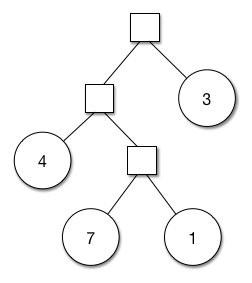
\includegraphics[width=.3\framewidth]{tree.png}
\end{center}
}

\onslide+<3->
\de{Summenfunktion}\en{Summary function}:
\onslide+<4->
\begin{lstlisting}{Haskell}
treeSum	(Leaf x) = x
\end{lstlisting}
\onslide+<5->
\vspace{-1.1em}
\begin{lstlisting}{Haskell}
treeSum (Node m n) = treeSum m + treeSum n
\end{lstlisting}
\onslide+<6->
\begin{lstlisting}{Haskell}
treeSum myTree                                -- 15
\end{lstlisting}
\end{frame}


%%%%%%%%%%%%%%%%%%%%%%%%%%%%%%%%%%%%%%%%%%%%%%%%%%
% Unterschiedlich!!
\begin{frame}[fragile]{\de{Fazit}\en{Bottom line}}
\begin{itemize}
\item \de{Funktionale Programmierung ist verbreiteter als man denkt}\en{Functional programming is more common than you may have expected}
% \item Java 8 \de{hat funktionale Neuerungen}\en{has new functional features}
\item \de{Manches lässt sich in den nicht-funktionalen Alltag integrieren}\en{Some of it can be integrated into non-functional coding}
\item \de{Viele Sprachen bringen funktionale Aspekte oder Zusatzmodule mit}\en{Many languages have functional aspects or additional modules}
\end{itemize}

\vfill

\onslide+<2->
\de{Referenz}\en{Reference}:

\begin{itemize}
\item Haskell: \url{http://www.haskell.org}
\end{itemize}

\end{frame}




%%%%%%%%%%%%%%%%%%%%%%%%%%%%%%%%%%%%%%%%%%%%%%%%%%
{
\begin{frame}{\de{Vielen Dank!}\en{Thank you very much!}}

        Code \& \de{Folien auf}\en{slides on} GitHub:
        \begin{center}
                \url{https://github.com} \url{/NicoleRauch/FunctionalProgrammingForBeginners}
        \end{center}

        ~\\[1em]
        \begin{block}{Nicole Rauch}
        \begin{description}[Twitterxx]
                \item[E-Mail]  \href{mailto:info@nicole-rauch.de}{\texttt{info@nicole-rauch.de}}
                \item[Twitter] \href{http://twitter.com/NicoleRauch}{\texttt{@NicoleRauch}}
                \item[Web] \href{http://www.nicole-rauch.de}{\texttt{http://www.nicole-rauch.de}}
        \end{description}
        \end{block}
        
        \de{
        \begin{itemize}
	\item Artikel in der nächsten (?) Java Aktuell
	\item Ganztägiger Workshop
	\end{itemize}
	}
\end{frame}
}
